% This is the Reed College LaTeX thesis template. Most of the work
% for the document class was done by Sam Noble (SN), as well as this
% template. Later comments etc. by Ben Salzberg (BTS). Additional
% restructuring and APA support by Jess Youngberg (JY).
% Your comments and suggestions are more than welcome; please email
% them to cus@reed.edu
%
% See https://www.reed.edu/cis/help/LaTeX/index.html for help. There are a
% great bunch of help pages there, with notes on
% getting started, bibtex, etc. Go there and read it if you're not
% already familiar with LaTeX.
%
% Any line that starts with a percent symbol is a comment.
% They won't show up in the document, and are useful for notes
% to yourself and explaining commands.
% Commenting also removes a line from the document;
% very handy for troubleshooting problems. -BTS

% As far as I know, this follows the requirements laid out in
% the 2002-2003 Senior Handbook. Ask a librarian to check the
% document before binding. -SN

%%
%% Preamble
%%
% \documentclass{<something>} must begin each LaTeX document
\documentclass[12pt,twoside]{reedthesis}
% Packages are extensions to the basic LaTeX functions. Whatever you
% want to typeset, there is probably a package out there for it.
% Chemistry (chemtex), screenplays, you name it.
% Check out CTAN to see: https://www.ctan.org/
%%
\usepackage{graphicx,latexsym}
\usepackage{amsmath}
\usepackage{amssymb,amsthm}
\usepackage{longtable,booktabs,setspace}
\usepackage{chemarr}%% Useful for one reaction arrow, useless if you're not a chem major
\usepackage[hyphens]{url}
% Added by CII
\usepackage{hyperref}
\usepackage{lmodern}
\usepackage{float}
\floatplacement{figure}{H}
% Thanks, @Xyv
\usepackage{calc}
% End of CII addition
\usepackage{rotating}


% Next line commented out by CII
%%% \usepackage{natbib}
% Comment out the natbib line above and uncomment the following two lines to use the new
% biblatex-chicago style, for Chicago A. Also make some changes at the end where the
% bibliography is included.
%\usepackage{biblatex-chicago}
%\bibliography{thesis}


% Added by CII (Thanks, Hadley!)
% Use ref for internal links
\renewcommand{\hyperref}[2][???]{\autoref{#1}}
\def\chapterautorefname{Chapter}
\def\sectionautorefname{Section}
\def\subsectionautorefname{Subsection}
% End of CII addition

% Added by CII
\usepackage{caption}
\captionsetup{width=5in}
% End of CII addition



% \usepackage{times} % other fonts are available like times, bookman, charter, palatino

% Syntax highlighting #22

% To pass between YAML and LaTeX the dollar signs are added by CII
\title{Bayesian Hierarchial Modeling of Historical Irrigaiton Patterns}
\author{Rachel Ledig}
% The month and year that you submit your FINAL draft TO THE LIBRARY (May or December)
\date{December 2021}
\division{Albrecht Daniel Thaer Institute for Agricultural and Horticultural Sciences}
\advisor{Dr.~Tobias Krueger}
\institution{University of Humboldt}
\degree{Master of Science}
\bday{Nov 17, 1991}
\bplace{California, USA}
\matriculation{602220}
\email{\href{mailto:ledigrac@hu-berlin.de}{\nolinkurl{ledigrac@hu-berlin.de}}}
%If you have two advisors for some reason, you can use the following
% Uncommented out by CII
\altadvisor{Dr.~Christian Schleyer}
\supervisor{Dr.~Fabian Stenzel}
% End of CII addition

%%% Remember to use the correct department!
\department{Faculty of Life Sciences}
% if you're writing a thesis in an interdisciplinary major,
% uncomment the line below and change the text as appropriate.
% check the Senior Handbook if unsure.
%\thedivisionof{The Established Interdisciplinary Committee for}
% if you want the approval page to say "Approved for the Committee",
% uncomment the next line
%\approvedforthe{Committee}

% Added by CII
%%% Copied from knitr
%% maxwidth is the original width if it's less than linewidth
%% otherwise use linewidth (to make sure the graphics do not exceed the margin)
\makeatletter
\def\maxwidth{ %
  \ifdim\Gin@nat@width>\linewidth
    \linewidth
  \else
    \Gin@nat@width
  \fi
}
\makeatother

% From {rticles}
\newlength{\csllabelwidth}
\setlength{\csllabelwidth}{3em}
\newlength{\cslhangindent}
\setlength{\cslhangindent}{1.5em}
% for Pandoc 2.8 to 2.10.1
\newenvironment{cslreferences}%
  {}%
  {\par}
% For Pandoc 2.11+
% As noted by @mirh [2] is needed instead of [3] for 2.12
\newenvironment{CSLReferences}[2] % #1 hanging-ident, #2 entry spacing
 {% don't indent paragraphs
  \setlength{\parindent}{0pt}
  % turn on hanging indent if param 1 is 1
  \ifodd #1 \everypar{\setlength{\hangindent}{\cslhangindent}}\ignorespaces\fi
  % set entry spacing
  \ifnum #2 > 0
  \setlength{\parskip}{#2\baselineskip}
  \fi
 }%
 {}
\usepackage{calc} % for calculating minipage widths
\newcommand{\CSLBlock}[1]{#1\hfill\break}
\newcommand{\CSLLeftMargin}[1]{\parbox[t]{\csllabelwidth}{#1}}
\newcommand{\CSLRightInline}[1]{\parbox[t]{\linewidth - \csllabelwidth}{#1}}
\newcommand{\CSLIndent}[1]{\hspace{\cslhangindent}#1}

\renewcommand{\contentsname}{Table of Contents}
% End of CII addition

\setlength{\parskip}{0pt}

% Added by CII

\providecommand{\tightlist}{%
  \setlength{\itemsep}{0pt}\setlength{\parskip}{0pt}}

\Acknowledgements{

}

\Dedication{
To Mom, Dad, Sis, and Fi.
}

\Preface{

}

\Abstract{
The preface pretty much says it all.

\par

Second paragraph of abstract starts here.
}

\Abbreviations{
\begin{tabular}{rp{0.2cm}lp{1cm}rp{0.2cm}l} IF & &  Irrigation Fraction \\ DAG & &  Directed Acyclic Graph \\ TRI & & Terrain Ruggedness Index \\ DEM & & Digital Elevation Model \\ \end{tabular}
}

	\usepackage{wrapfig}
	\usepackage{booktabs}
 \usepackage{longtable}
 \usepackage{array}
 \usepackage{multirow}
 \usepackage{wrapfig}
 \usepackage{float}
 \usepackage{colortbl}
 \usepackage{pdflscape}
 \usepackage{tabu}
 \usepackage{threeparttable}
 \usepackage{threeparttablex}
 \usepackage[normalem]{ulem}
 \usepackage{makecell}
 \usepackage{xcolor}
% End of CII addition
%%
%% End Preamble
%%
%
\begin{document}

% Everything below added by CII
  \maketitle

\frontmatter % this stuff will be roman-numbered
\pagestyle{empty} % this removes page numbers from the frontmatter



  \hypersetup{linkcolor=black}
  \setcounter{secnumdepth}{2}
  \setcounter{tocdepth}{2}
  \tableofcontents


  \listoftables

  \listoffigures
  \begin{abbreviations}
    \begin{tabular}{rp{0.2cm}lp{1cm}rp{0.2cm}l} IF & &  Irrigation Fraction \\ DAG & &  Directed Acyclic Graph \\ TRI & & Terrain Ruggedness Index \\ DEM & & Digital Elevation Model \\ \end{tabular}
  \end{abbreviations}
  \begin{abstract}
    The preface pretty much says it all.

    \par

    Second paragraph of abstract starts here.
  \end{abstract}
  \begin{dedication}
    To Mom, Dad, Sis, and Fi.
  \end{dedication}
\mainmatter % here the regular arabic numbering starts
\pagestyle{fancyplain} % turns page numbering back on

\hypertarget{intro}{%
\chapter{Introduction}\label{intro}}

The practice of irrigation, and its subsequent impacts, have far reaching effects for the global economy, food and water supply, and environment. Irrigated land accounts for 20\% of the global cultivated land area which derives 40\% of the global food supply \protect\hyperlink{ref-portmannMIRCA2000GlobalMonthly2010a}{Portmann, Siebert, \& Döll} (\protect\hyperlink{ref-portmannMIRCA2000GlobalMonthly2010a}{2010}), 70\% of water withdrawls from ground water aquifers are used for irrigation (\protect\hyperlink{ref-faoStateWorldLand2011}{FAO, 2011}), and

\hypertarget{objectives}{%
\section{Objectives}\label{objectives}}

Ultimately, the agricultural system will continue to demand more water while competing with other sectors over decreasing water availability in the coming years. With this pressure, farmers will aim to be as efficient as possible by increasing their yields which, in certain areas and under certain conditions, can be done by irrigating their fields. Understanding where, when, and why farmers decide to begin irrigating is important to understand water demands now and in the future. Unfortunately, irrigation expansion is seldom studied, with few studies using statistical modeling techniques to investigate the role that biophysical, economic, and political factors play in the spread of irrigation infrastructure in the present. None do so historically. This leads to the first and overarching research question:

\emph{Which factors (drivers) have influenced the expansion of irrigation in both time and space over the past 100 years?}

By understanding under which conditions irrigation infrastructure is built could be coupled with projections of future climate and economic scenarios, allowing us to get a better idea of scales of agricultural production, land use, and water needs in the coming years. In order to eventually extrapolate to the future, predictive accuracy needs to be addressed. This can be done by separating data into training and testing datasets, model tuning, and error estimation.

Several other questions smaller questions arise in regard to drivers of expansion which are interesting to investigate. Such as:
\begin{itemize}
\item
  Which has a larger influence on irrigation expansion patterns, biophysical or socio-economic factors?
\item
  Do rates of irrigation expansion differ depending on crop type?
\end{itemize}
Both of these questions have interesting policy implications, should large trends be present in the model and analysis.

The time series component of this data set also gives rise to some interesting questions.
\begin{itemize}
\item
  Expansion rates of total irrigated area differ temporally, what could be the drivers for this difference?
\item
  Is there a temporal delay in irrigation expansion based on the influence of certain drivers, and if so how much?
\end{itemize}
\hypertarget{Theory}{%
\chapter{Context}\label{Theory}}

This chapter details the theoretical basis for this thesis. Initially, literature will be reviewed beginning with irrigation expansion drivers in Section \ref{drivers} and followed by a detailed account of prior irrigation modeling studies in Section \ref{irrmodslit}. Finally, an account of the basics of Bayesian inference will be described in Section \ref{bayesintro}.

\hypertarget{irrmodslit}{%
\section{Modeling Studies of Irrigation Expansion}\label{irrmodslit}}

Shifting gears, there are few studies that investigate the drivers or irrigation expansion. Those that do, only one takes in to account historical data or detail expansion rates based on regions or countries. \protect\hyperlink{ref-siebertGlobalDataSet2015}{Stefan Siebert et al.} (\protect\hyperlink{ref-siebertGlobalDataSet2015}{2015}), after collecting a global dataset of historical irrigation patterns, goes on to investigate trends and patterns in global irrigation. The authors note that rates of irrigation expansion can be divided into two main time periods, before and after 1950, documenting that from 1900 to 1950 global irrigation doubled and from 1950 to 2005 global irrigated area tripled. Different regions also experienced different growth rates, with regions such as Australia and Oceania, southeastern Asia, Middle and South Africa, Central America, and eastern Asia experiencing growth rates higher than that of the global average and the North of Africa and North America, experiencing lower than average growth rates. Europe and Western Asia also stand out here with a slow decrease of area equipped for irrigation seen toward the end of the study period, confirming what \protect\hyperlink{ref-angelakisIrrigationWorldAgricultural2020}{Angelakis et al.} (\protect\hyperlink{ref-angelakisIrrigationWorldAgricultural2020}{2020}) mentions regarding the disintegration of irrigation schemes after the dissolution of the USSR. In general \protect\hyperlink{ref-siebertGlobalDataSet2015}{Stefan Siebert et al.} (\protect\hyperlink{ref-siebertGlobalDataSet2015}{2015}) conclude that in 1900 irrigation took place predominately in arid locations, which expanded into more humid climes as the study period progresses, in fact, the percentage of global irrigation that occurred in arid regions remained relatively stable from 1900 to 2005, as where the percentage of global area equipped for irrigation went down in areas with rice cultivation and up in other wet areas. Ultimately, \protect\hyperlink{ref-siebertGlobalDataSet2015}{Stefan Siebert et al.} (\protect\hyperlink{ref-siebertGlobalDataSet2015}{2015}) connect changes in irrigation to several variables including population, aridity, and river discharge.

\protect\hyperlink{ref-neumannExploringGlobalIrrigation2011}{Neumann et al.} (\protect\hyperlink{ref-neumannExploringGlobalIrrigation2011}{2011}) attempt to model current irrigation patterns based on a variety of biophysical factors (slope, discharge, humidity, ET, evap, pop density, etc) and political factors (democracy, GDP, corruption, political stability) at two different levels, grid cell (5 arc-minute grid cells) and at a country level. However, Neumann's study is only modeling the current irrigation pattern, with no historical perspective. The authors find that the addition of socio-economic information to the model does help improve the explanation the current irrigation pattern, but not only to a small extent. A delay existed, as current patterns are formed from decisions, policies, and economic conditions that occurred years before.

\protect\hyperlink{ref-puyCurrentModelsUnderestimate2020}{Puy, Lo Piano, \& Saltelli} (\protect\hyperlink{ref-puyCurrentModelsUnderestimate2020}{2020}) discuss uncertainties of published projected irrigation expansion patterns by comparing these projections to a simple model that predicts irrigated area as a function of only population size, bounded by available water and land. A simple model was constructed for ease of interpretation, as the main purpose of this study is to discuss uncertainties present in this (seemingly) simple model and investigate how other published projections of irrigation expansion fall within \protect\hyperlink{ref-puyCurrentModelsUnderestimate2020}{Puy, Lo Piano, \& Saltelli} (\protect\hyperlink{ref-puyCurrentModelsUnderestimate2020}{2020})'s model's range of uncertainty. \protect\hyperlink{ref-puyCurrentModelsUnderestimate2020}{Puy, Lo Piano, \& Saltelli} (\protect\hyperlink{ref-puyCurrentModelsUnderestimate2020}{2020})'s justification for modeling irrigated area as a function of only population size stems from the previous studies showing that population is a variable that encapsulates much more complicated socio-ecological relationships.

\hypertarget{drivers}{%
\section{Establishing a Framework for Irrigation Expansion}\label{drivers}}

\hypertarget{drivers-1}{%
\subsection{Drivers}\label{drivers-1}}

Understanding the mechanisms behind irrigation and the features of irrigation systems is imperative to understanding why, when, and where irrigation is implemented. According to the \protect\hyperlink{ref-faoGuidelinesDesigningEvaluating1989}{FAO \& Walker} (\protect\hyperlink{ref-faoGuidelinesDesigningEvaluating1989}{1989}), the choice by the farmer of irrigation technology is dependent on several intertwined socio-economic and biophysical concerns. Multitudes of literature exist detailing the considerations necessary when choosing an irrigation system, but little exists on why farmers choose to irrigate in the first place. Although the distinction is notable and directly equating the choice of a specific irrigation technology to the decision to begin irrigating is perhaps naive, it is important to understand that the decision to irrigate \emph{is not possible} without the simultaneous choice of an irrigation technology. Therefore using the irrigation technology selection criteria outlined by \protect\hyperlink{ref-faoGuidelinesDesigningEvaluating1989}{FAO \& Walker} (\protect\hyperlink{ref-faoGuidelinesDesigningEvaluating1989}{1989}) as a basis to discuss drivers of irrigation expansion is justified.

By using these areas as a guideline for what farmers are concerned about when establishing an irrigation system and why those concerns exist, not only can the causal relationship between external conditions and irrigation expansion be investigated, but appropriate predictors for the hierarchical model can also be selected. These eight components are detailed in the subsections below.

To begin, it is important to know a little bit about irrigation systems. Irrigation systems can be divided into two main systems: gravity fed which includes all types of surface irrigation, and mechanized pump systems, such as sprinkler or localized distributions (\protect\hyperlink{ref-bjornebergIRRIGATIONMethods2013}{Bjorneberg, 2013}). Surface irrigation, such as furrow, basin, or border irrigation, is the oldest, simplest, and cheapest method available and used on around 85\% of the irrigated land in the world (\protect\hyperlink{ref-bjornebergIRRIGATIONMethods2013}{Bjorneberg, 2013}; \protect\hyperlink{ref-holzapfelIrrigationAgriculture2008}{Holzapfel \& Mariño, 2008}). Pumped irrigation systems are less common globally. Different types of irrigation can be seen in Figure \ref{fig:irrigationtypes}.
\begin{figure}

{\centering 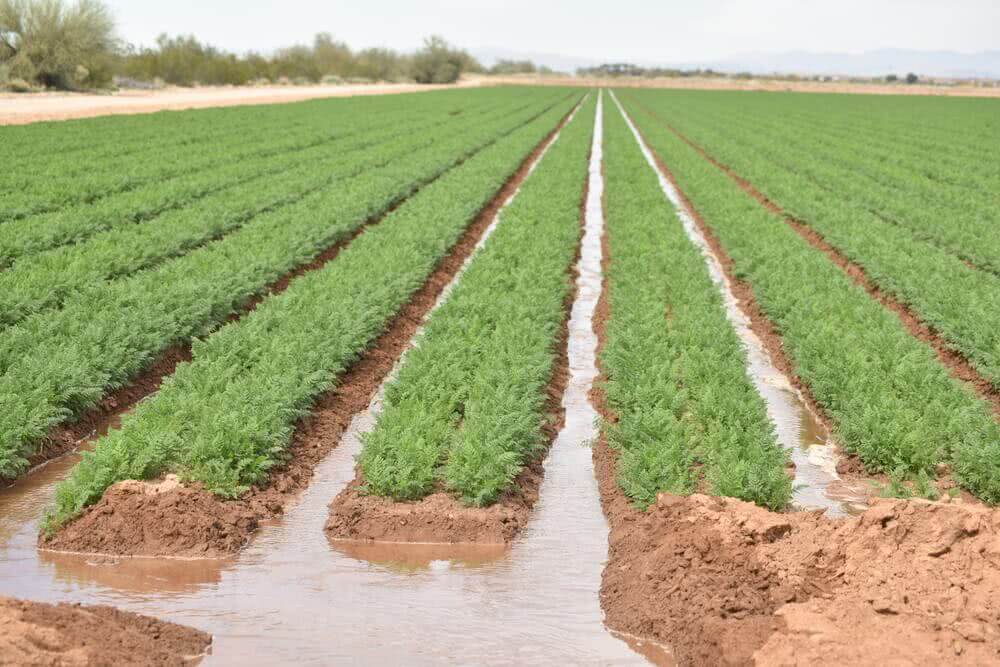
\includegraphics[width=0.3\linewidth,height=0.2\textheight]{figure/FurrowPic} 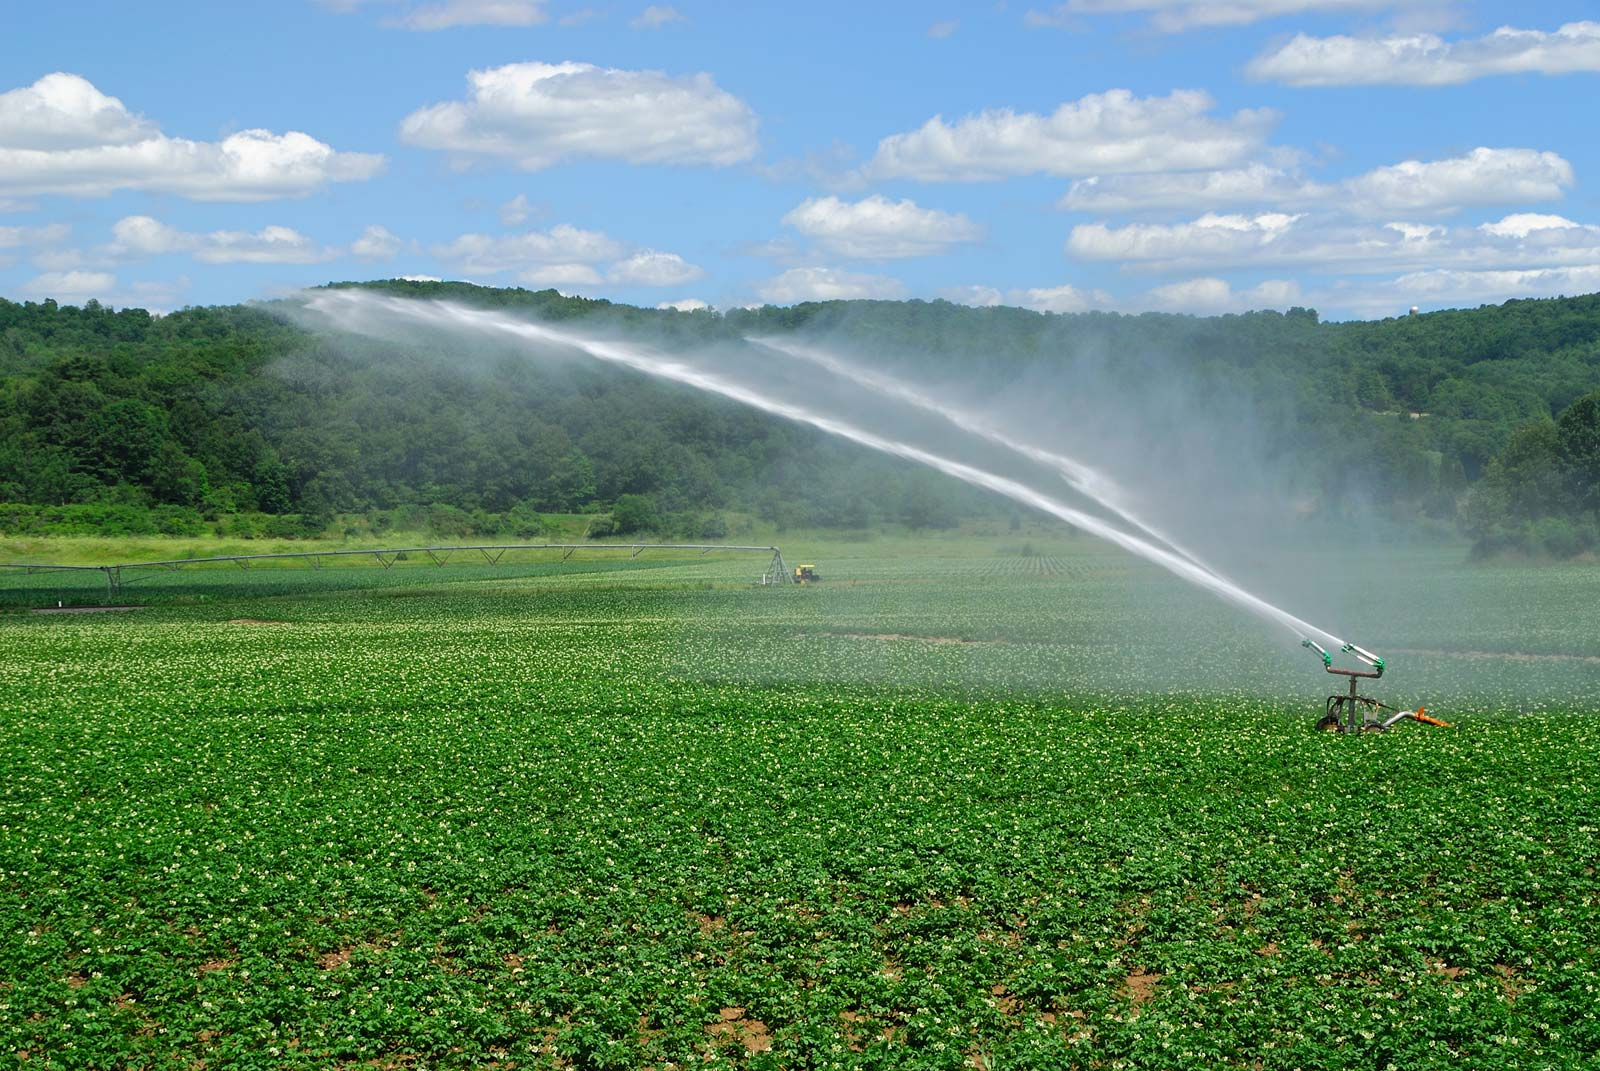
\includegraphics[width=0.3\linewidth,height=0.2\textheight]{figure/Irrigation-sprinklers} 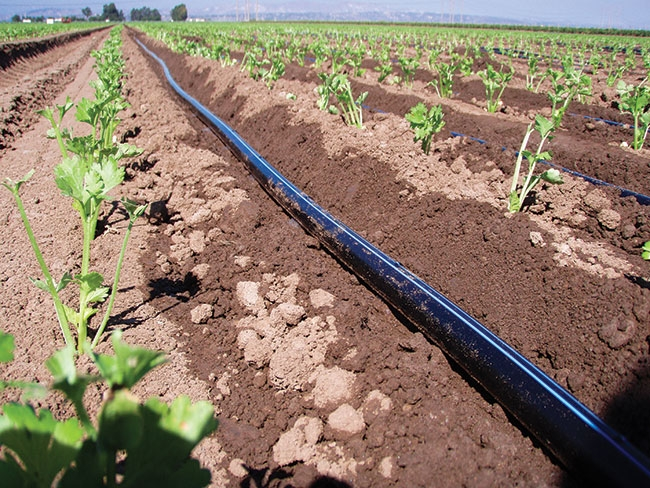
\includegraphics[width=0.3\linewidth,height=0.2\textheight]{figure/DripIrrigation} 

}

\caption{Furrow, Sprinkler and Drip irrigation  [@GoogleImages2021]}\label{fig:irrigationtypes}
\end{figure}
\hypertarget{water}{%
\subsubsection{Water}\label{water}}

Water supply is a core component of irrigation and can be divided into two main dimensions, water quantity, and water quality. As water quality matters more for the choice of a specify irrigation technology, it will not be discussed in detail below. Water quantity, however, is a large concern when deciding if a farmer can irrigate. In the natural world, water comes from three sources: rain, surface water (rivers, lakes, reservoirs, etc.), or groundwater (aquifers).

Precipitation, specifically rainfall, is not technically an irrigation water source as is applied directly to crops without any irrigation system. As a result, rainfall, a free source of crop water, currently sustains roughly 80\% of the global cultivated area which produces 60\% of the total crop production (\protect\hyperlink{ref-worldwaterassesnentprogramUnitedNationsWorld2009}{Program \& UNESCO, 2009}). Although direct rainfall is the predominant method for watering crops and can nullify the need for any irrigation technology, meeting crop water demand with rainfall can be difficult as rainfall can be extremely varied in both space and time. Spatially, different regions receive different annual amounts of rainfall, with tropical and temperate zones receiving more rainfall than semi-arid or arid regions (\protect\hyperlink{ref-forsethTerrestrialBiomes2010}{Forseth, 2010}). However, mean annual rainfall does not show the whole picture, and when deciding whether the amount of precipitation in a region is sufficient to sustain crop growth, it is important to remember that rainfall can heavily vary in seasonality, as well. Wet and dry seasons dictate the boom and bust of vegetation in some tropical and sub-tropical regions {[}CITATION{]}. The coincidence of rainfall and crop growing season is integral for farmers as crop water demands must be met during the specific periods of the crop's growing cycle. One benefit of rain-fed agriculture is that rainwater is naturally of high quality, meaning that it is free of solids and harmful substances that other water sources may have (\protect\hyperlink{ref-douglascoxWaterQualityCrop2015}{\textbf{douglascoxWaterQualityCrop2015?}}). Although, it should be noted that patterns of rainfall are shifting with the effects of climate change. When long-standing climactic patterns change, differences in annual rainfall amounts, duration of the wet and dry seasons, and intensity of rainfall have consequences for both farmers and crops, making planning for a productive growing season more difficult in some areas (\protect\hyperlink{ref-rockstromManagingWaterRainfed2010}{Rockström et al., 2010}). These changes have the potential to incentivize the shift from rainfed agriculture to irrigated.

Surface water is only applied to crops through an irrigation system, unlike rainwater. Surface water is water that is collected, from precipitation, runoff, and up-welling of groundwater resources, on the surface of the planet (in rivers, lakes, ponds, and dams). Surface water is the most common water source for irrigation as its supply is generally less variable than precipitation and easier to access than groundwater. As a result, 54\% of the area available for irrigation is irrigated with surface water (\protect\hyperlink{ref-siebertGroundwaterUseIrrigation2010}{S. Siebert et al., 2010}; \protect\hyperlink{ref-thenkabailGlobalIrrigatedArea2009}{Thenkabail et al., 2009}). Surface water, due to the fact that it is accumulative, potentially passes through many environments before it is extracted by the farmer and applied to the field, meaning that issues with water quality are more common. Pollution, sediment, and salts must be monitored to ensure that the surface water can be applied to crops and is able to pass through the specific irrigation distribution system (\protect\hyperlink{ref-faoIrrigationManualPlanning2001}{FAO \& SAFR, 2001}). Again, it should be pointed out that since the original source of most surface water is precipitation in some form, it is also susceptible to changes in precipitation patterns due to climate change.

Groundwater, water that is stored below ground in aquifers, is a collection of water that has infiltrated through the soil over many years. As a source of clean reliable irrigation water, groundwater is unparalleled (\protect\hyperlink{ref-siebertGroundwaterUseIrrigation2010}{S. Siebert et al., 2010}). The water stored in aquifers is of high quality and much more resistant to seasonal changes in precipitation than surface water. Groundwater's largest issue, with respect to its use as a source of water for irrigation, is access. Multiple methods for groundwater extraction exist but most are more costly than surface water withdrawals. However, in semi-arid or arid regions where surface water may also be seasonal or non-existent, extraction of groundwater for irrigation becomes more economically viable as its use can sustain large populations (E.g. regions in the middle east).

Ultimately, rainfall is always the default source for farmers to supply water to their crops, and only when rainfall is not sufficient during necessary parts of the crop growing season, do farmers consider using irrigation to meet the crop water demand.

\hypertarget{topo}{%
\subsubsection{Topography}\label{topo}}

Steep topography can prevent the implementation of the majority of most common and basic surface irrigation systems, such as furrow (using long channels to water crops) or basin (flooding of field sections) irrigation. Generally, for this type of irrigation to be used field slopes need to have less than a 5\% incline, which limits the application of this simple type of irrigation to valleys and flatlands (\protect\hyperlink{ref-faoIrrigationManualPlanning2001}{FAO \& SAFR, 2001}).

Other types of irrigation, sprinkler or localized systems, can be utilized in steeper environments, but are often more costly than simple surface irrigation techniques. There are some ingenious examples of farmers working with topography to use simple irrigation methods and adapt to steeper slopes: rice terraces in South East Asia use basin irrigation to cultivate paddy rice on extremely steep slopes (\protect\hyperlink{ref-adachiAgriculturalTechnologiesTerraced2007}{Adachi, 2007}). However, in general, steep slopes are rarely irrigated with surface irrigation methods.

\hypertarget{soil}{%
\subsubsection{Soil}\label{soil}}

Soil composition, in the context of irrigation, is important because different soils have different capacities to store and infiltrate water, meaning that different types of irrigation systems may be necessary to ensure that crops are able to get the water that they need (\protect\hyperlink{ref-faoGuidelinesDesigningEvaluating1989}{FAO \& Walker, 1989}). For example, sandy soils retain less water and drain faster, meaning that they must be irrigated more frequently but with less water. In this case, surface irrigation methods that apply large amounts of water to a field at one time may be less suited for these soils (\protect\hyperlink{ref-faoIrrigationWaterManagement1986a}{FAO, Brouwer, \& Heibloem, 1986}). In addition, as the soil type dictates the infiltration rate of irrigation water and therefore the rate of application, the soil type combined with the specific irrigation method chosen may impose requirements on the consistency and volume of the water supply. For the context of this thesis, soil composition will be largely ignored as the oftentimes soil composition limits the type of irrigation used, not the absence or presence of it. However, it is important to note that as surface irrigation methods, which are more common worldwide, are less suitable for certain soil types (E.g. sandy soils), there may be circumstances in which given a specific soil type, irrigation would be inefficient.

\hypertarget{crops}{%
\subsubsection{Crops}\label{crops}}

Crop type also has the potential to influence the presence/absence of irrigation and the type used as different crops require different amounts of water over the the growing period (\protect\hyperlink{ref-faoIrrigationWaterManagement1986}{FAO, Brouwer, Prins, Kay, \& Heibloem, 1986}). Staple crops that need to be irrigated are rarely irrigated with sprinkler or localized (drip) systems as these systems are much more costly than surface irrigation. Sprinkler and localized systems are almost always reserved for fruits and vegetables, so-called cash crops (\protect\hyperlink{ref-faoIrrigationWaterManagement1985}{FAO, Brouwer, Goffeau, \& Heibloem, 1985}).

\hypertarget{combatibility}{%
\subsubsection{Compatibility}\label{combatibility}}

Irrigation technologies must be a benefit not a burden to the farmer and the choice to irrigate must fit within the given growing and harvesting needs of a particular crop. Irrigation must not impede the usage of pruning or harvesting machinery (\protect\hyperlink{ref-faoGuidelinesDesigningEvaluating1989}{FAO \& Walker, 1989}). In addition, the farmers must be able to work with the chosen irrigation technology. Sprinkler and localized systems are more complicated than surface irrigation, however, surface irrigation requires more manual input from the farmer. Surface irrigation is also easier to maintain than other types of irrigation (\protect\hyperlink{ref-faoIrrigationWaterManagement1986a}{FAO, Brouwer, \& Heibloem, 1986}). This is less of a concern for this thesis, as compatibility issues between crop type, irrigation system, farmer knowledge, and other farm machinery is not the main focus.

\hypertarget{econ}{%
\subsubsection{Economics}\label{econ}}

The economics of specific irrigation systems and the choice to irrigate is important for farmers, as even the simplest surface irrigation methods are not without costs. Water, energy, materials, labor, maintenance, and monitoring costs must all be considered when deciding to begin irrigating and which irrigation system to choose (\protect\hyperlink{ref-faoGuidelinesDesigningEvaluating1989}{FAO \& Walker, 1989}). According to \protect\hyperlink{ref-faoIrrigationManualPlanning2001}{FAO \& SAFR} (\protect\hyperlink{ref-faoIrrigationManualPlanning2001}{2001}), for small farms in Sub-Saharan Africa, up to 80\% of the costs to develop an irrigation system stems from water resource procurement, such as construction of a dam. In addition, the authors note that the cost for cubic meter of water is increasing in this region as well, putting more economic pressure on the farmers.

\hypertarget{socinf}{%
\subsubsection{Social Influences}\label{socinf}}

However, there are ways to shift the costs of establishing irrigation from the individual farmer to the collective. Grass-roots, bottom-up irrigation cooperatives or schemes may be set up to share the construction, maintenance, and monitoring of shared irrigation and water transportation infrastructure (\protect\hyperlink{ref-faoGuidelinesDesigningEvaluating1989}{FAO \& Walker, 1989}). \protect\hyperlink{ref-faoGuidelinesDesigningEvaluating1989}{FAO \& Walker} (\protect\hyperlink{ref-faoGuidelinesDesigningEvaluating1989}{1989}) note that there are often several levels involved in the organization of irrigation schemes. These include the individual farmers who participate at the field level; the local farmers' collectives who manage operation, maintenance, allocation, and conflicts; the governing body at the local or state level that deals with water distribution and funding. Each actor has different needs, power, and roles ensuring the management of local irrigation. Examples of irrigation schemes are common globally and historically.

\hypertarget{extinf}{%
\subsubsection{External Influences}\label{extinf}}

Sometimes external factors play a large role in stimulating irrigation expansion. Social trends, governmental programs, and conflicts among others can influence the rate of irrigation expansion at a sub-national, national, or regional level. This type of expansion could be labeled as top-down, as generally there are larger actors pushing or incentivising the construction of irrigation infrastructure, in comparison to the bottom-up dynamic of locally organized irrigation schemes.

\protect\hyperlink{ref-angelakisIrrigationWorldAgricultural2020}{Angelakis et al.} (\protect\hyperlink{ref-angelakisIrrigationWorldAgricultural2020}{2020}) details explicitly some of these trends that have occurred during the last century. In Spain, during the reign of Francisco Franco,\footnote{At the equator, this is roughly a 9.2km by 9.2km grid cell resolution.} the government began a national water development plan to settle small farmers. This campaign created the foundation for Spain's expansive irrigated agricultural system today, the largest irrigated area in the European Union. Another instance that \protect\hyperlink{ref-angelakisIrrigationWorldAgricultural2020}{Angelakis et al.} (\protect\hyperlink{ref-angelakisIrrigationWorldAgricultural2020}{2020}) discusses is the sudden overall increase in irrigated area after the Second World War, which is attributed to two aspects: a sudden population increase and developments in technology. The population increase, due to increased birthrates and an extension of life span due to medical advances, created a demand for more food and advances in technology, specifically those that were necessary to optimize pumps needed for pressurized irrigation and water transportation systems. Both of these changes resulted in a rapid global expansion of irrigated area. Other examples exist such as the Green Revolution, or Third Agricultural Revolution,\footnote{The act of harvesting rainwater during rain and then later applying it to crops.} also spurred trends of irrigation expansion, particularly in Asia (\protect\hyperlink{ref-angelakisIrrigationWorldAgricultural2020}{Angelakis et al., 2020}). \protect\hyperlink{ref-angelakisIrrigationWorldAgricultural2020}{Angelakis et al.} (\protect\hyperlink{ref-angelakisIrrigationWorldAgricultural2020}{2020}) points out that large scale irrigation projects often succeed due to governmental involvement and support from changing market patterns.

\bigskip

Ultimately, the drivers of irrigation are complex and interconnected. When quantifying these forces behind an ever changing pattern of irrigation it is easy to generalize, but the reality of irrigation is that there are infinite combinations of conditions, contexts, times, and ambitions that determine the ultimate success or failure of an irrigation project. What worked in one place and time, is not guaranteed to result in a positive outcome years later and worlds apart. The above sections are not exhaustive in their description of the complexity that is involved in the planning, construction, and operation of the majority of irrigation projects, but they are a good start.

\hypertarget{section}{%
\section{}\label{section}}

\hypertarget{methods}{%
\chapter{Methods}\label{methods}}

\hypertarget{data}{%
\section{Data}\label{data}}

To appropriately choose data that encapsulates the concepts and relationships described in Section \ref{drivers} the following datasets and variables were collected and selected. It should be noted that many of these datasets contain more than one variable that would conceptually represent the links between expanding irrigation and various drivers. The predictors presented below were selected based on various reasons including data availability (both spatially and temporally) and conceptual fidelity. For more information on all potential variables please see Appendix Section \ref{predselect}.

\hypertarget{irrfrac}{%
\subsection{Outcome Variable: Irrigation Fraction}\label{irrfrac}}

\hypertarget{HID}{%
\subsubsection{Global Historical Irrigation Data Set}\label{HID}}

Data for global historical irrigation patterns was collected from the Global Historical Irrigation Data Set (HID) (\protect\hyperlink{ref-siebertGlobalDataSet2015}{Stefan Siebert et al., 2015}) which describes hectares of area equipped for irrigation (AEI) per grid cell at a 5 arcmin resolution\footnote{At the equator, this is roughly a 9.2km by 9.2km grid cell resolution.} over a period of 105 years, from 1900 to 2005. By documenting global and historical irrigation patterns, \protect\hyperlink{ref-siebertGlobalDataSet2015}{Stefan Siebert et al.} (\protect\hyperlink{ref-siebertGlobalDataSet2015}{2015}) hoped to create a better understanding of the evolution of said patterns. It is worth noting that the dataset provided in \protect\hyperlink{ref-siebertGlobalDataSet2015}{Stefan Siebert et al.} (\protect\hyperlink{ref-siebertGlobalDataSet2015}{2015}) documents area equipped for irrigation, meaning area that is equipped with infrastructure to irrigate crops but not \emph{necessarily} irrigated. In addition, rainwater harvesting\footnote{The act of harvesting rainwater during rain and then later applying it to crops.} is also not included in the summation of area equipped for irrigation. {[}CITATION{]}

To amass this data \protect\hyperlink{ref-siebertGlobalDataSet2015}{Stefan Siebert et al.} (\protect\hyperlink{ref-siebertGlobalDataSet2015}{2015}) used a variety of sources to collect national and subnational statistics including FAOSTAT (\protect\hyperlink{ref-faoFAOSTAT2021}{FAO, 2021b}), EuroStat (\protect\hyperlink{ref-europeancomissionEurostatDatabase2021}{Comission, 2021}), and Aquastat (\protect\hyperlink{ref-faoAQUASTAT2021}{FAO, 2021a}) along with other less collected sources like census data and statistical yearbooks. Data was recorded for 10 year timesteps until 1980 and five year timesteps until the termination of the study period in 2005. Data for the period prior to 1950 and for the year 2005 has higher levels of uncertainty in the measurements when compared to the data between 1950 and 2005, as irrigation data from international organizations (e.g.~FAO) were unavailable prior and post. After collection the data was harmonized and downscaled to a 5 arcmin resolution. Special care was taken to ensure that high resolution data (at a 5 arcmin resolution) could be accurately summed to the subnational level, ensuring accuracy at different resolutions. In addition, the authors note that validation of this dataset was not possible due to the fact that all available data was used as input to create the HID (\protect\hyperlink{ref-siebertGlobalDataSet2015}{Stefan Siebert et al., 2015}).

The HID, in combination with other datasets such the History Database of the Global Environment ( \protect\hyperlink{ref-kleingoldewijkHundredYear18901997}{Klein Goldewijk \& Battjes} (\protect\hyperlink{ref-kleingoldewijkHundredYear18901997}{1997}), see Section \ref{HYDE}) and Climate Research Unit Time Series Data ( \protect\hyperlink{ref-universityofeastangliaclimaticresearchunitVersionCRUTS2021}{University of East Anglia Climatic Research Unit, Harris, Osborn, \& Jones} (\protect\hyperlink{ref-universityofeastangliaclimaticresearchunitVersionCRUTS2021}{2021}), see Section (\protect\hyperlink{ref-ref}{\textbf{ref?}})(CRU)) were used was then fed into the LPJmL model. The Lund-Potsdam-Jena managed Land (LPJmL) is a Dynamic Global Vegetation Model which simulates the global terrestrial carbon cycle and the corresponding response of vegetation patterns, both natural and managed, under a given set of climactic conditions (\protect\hyperlink{ref-schaphoffLPJmL4DynamicGlobal2018}{Schaphoff et al., 2018}). Spatially and temporally explicit data regarding climate, landuse patterns, and anthropogenic activities among others is fed into the model and used to simulate, via the LPJmL's established biophysiological interconnections, a multitude of processes and outcome that relate to global vegetation patterns and carbon cycles(\protect\hyperlink{ref-pikLPJmLLundPotsdamJenaManaged}{PIK, n.d.}). For the purposes of this masters thesis, a global irrigation pattern represented by percentage of irrigated area per cell at a 0.5° x 0.5° latitude longitude global grid cell resolution with yearly observations for a period of 1960 to 2005 was extracted from the LPJmL model .

\hypertarget{irrfracdesc}{%
\subsubsection{Description}\label{irrfracdesc}}

Levels of irrigation vary widely both geographically and temporally. In Figure \ref{fig:irrfrac2005} the global irrigation pattern for the last year of they study period (2005) is depicted.
\begin{figure}
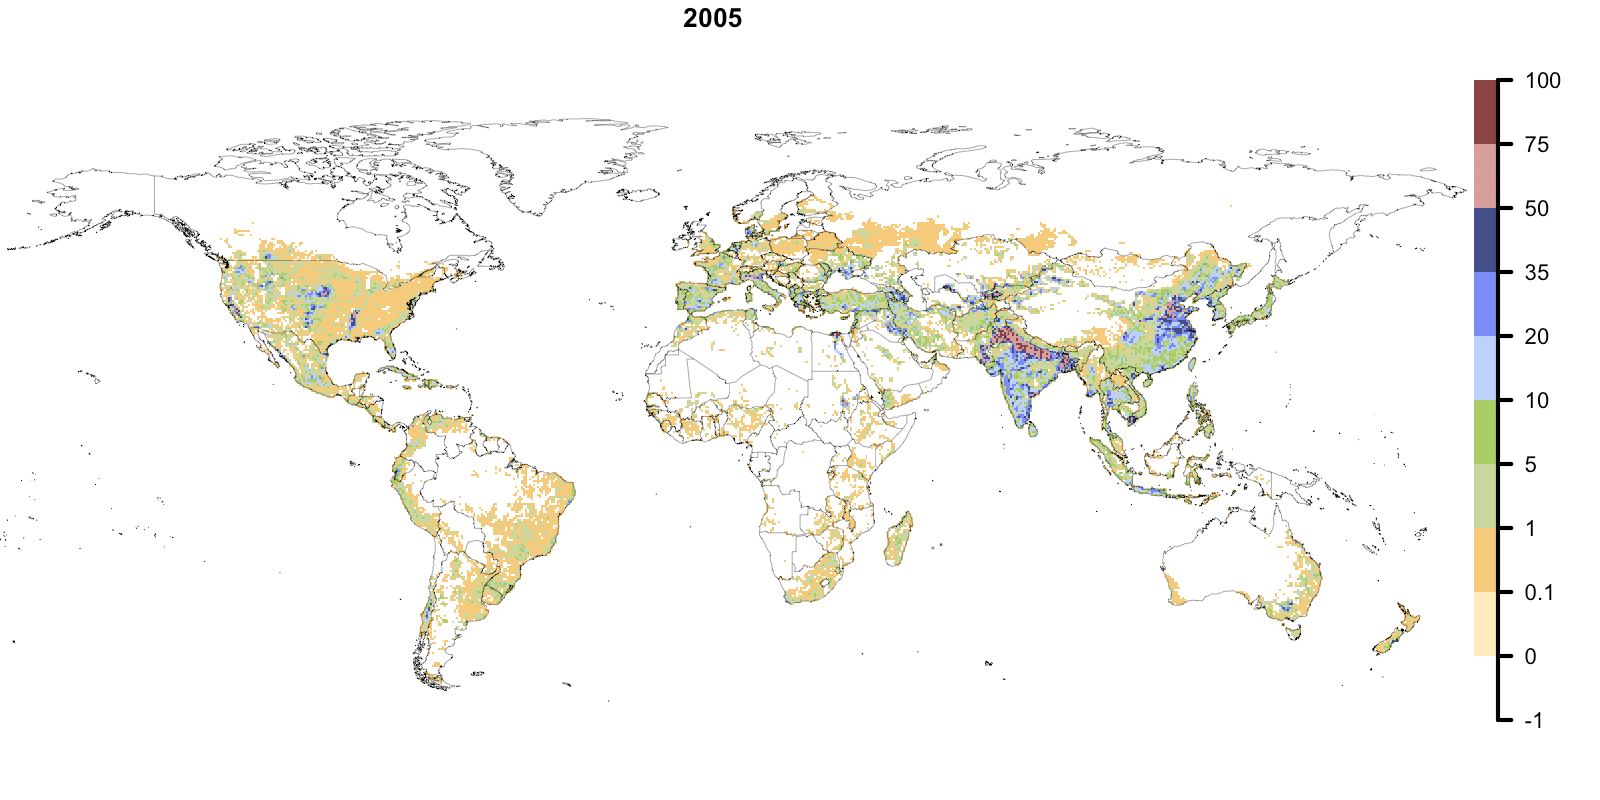
\includegraphics[width=1000px]{figure/irrfrac2005} \caption{Percentage of a cell's area covered by land equipped for irrigation. Represents the global irrigation pattern at a 0.5° x 0.5° latitude longitude grid cell resolution for the last year of the study period (2005).}\label{fig:irrfrac2005}
\end{figure}
There are several ``hotspots'' of irrigation that occur, predominantly in the interior of the United States, north of India, Bangladesh, and Eastern China in which more than 30\% of a cell is irrigated area. Otherwise, generally irrigation, where it exists, a small minority of cell area. No irrigation occurs in some places including towards arctic circle and in the Sahara, among other places.

When looking at the histogram of the data distribution of the target variable, irrigation fraction, it is clear to see that the data includes many zeros.

\hypertarget{precip}{%
\subsection{Water: Precipitation}\label{precip}}

To encapsulate the relationship between the presence/absence of irrigation or the amount of irrigation in a cell and water, precipitation was chosen to represent this link. Several other variables existed that would have also represented the connection between a water source and irrigation expansion, however to reduce multicollinearity, only one variable could be used to encapsulate all the effects of water. Through an iterative modeling process of checking the strength and stability of different predictor effects, precipitation was ultimately chosen. In addition, using precipitation as a predictor conveniently fits best within the conceptual framework better than others with the notion that farmers will begin to irrigate when there precipitation cannot meet crop demand.

\hypertarget{CRU}{%
\subsubsection{Climate Research Unit Time Series Dataset}\label{CRU}}

Data for precipitation was collected from the Climate Research Unit of the University of East Anglia. This dataset is open-source and includes monthly precipitation data for a 0.5° x 0.5° latitude longitude global grid cell resolution over a time period of 1901 to 2018. To collect this data, individual station observations were anomolized by using the each station's monthly mean from the years 1961 to 1990 to standardize observations as a percentage of the mean monthly value (value of -100 means 0 precipitation, value of 0 is equal to monthly mean for a given station). These anomolies were then converted to a 0.5° x 0.5° latitude longitude grid using angular distance weighting ultimately giving rise to a single monthly value for each grid cell (\protect\hyperlink{ref-universityofeastangliaclimaticresearchunitVersionCRUTS2021}{University of East Anglia Climatic Research Unit, Harris, Osborn, \& Jones, 2021}).

\hypertarget{precipdesc}{%
\subsubsection{Description}\label{precipdesc}}

Below

\hypertarget{rugged}{%
\subsection{Topography: Ruggedness}\label{rugged}}

In order to explain the relationship between topography and irrigation expansion, an index of a country's topographical heterogeniety was chosen. Other similar irrigation expansion studies similarly use slope (calculated from Digital Elevation Models (DEMs)) as a predictor for explaining irrigation expansion but do so using a 5 arcmin gridded slope dataset (\protect\hyperlink{ref-neumannExploringGlobalIrrigation2011}{Neumann et al., 2011}). Unfortunately for this thesis, grid cells used for analysis are significantly larger\footnote{A 5 arcmin global grid results in a 9.2km by 9.2km grid at the equator. This thesis uses a 0.5° x 0.5° lattitude longitude grid which produces a grid cell of about 55km by 55km at the equator.}, and an aggregation of slope to a larger grid cell was unfeasible for this thesis. Instead, a well know index of country topographical heterogeneity was chosen to represent the ``ruggedness'' of a country.

\hypertarget{TRI}{%
\subsubsection{Terrain Ruggedness Index}\label{TRI}}

The Terrain Ruggedness Index (TRI) was developed by \protect\hyperlink{ref-rileyTerrainRuggednessIndex1999}{Riley, Degloria, \& Elliot} (\protect\hyperlink{ref-rileyTerrainRuggednessIndex1999}{1999}) initially to be used to analyze the effects of topography on species habitats and behaviors. The authors developed a simple method to calculate the heterogeneity of a given area using DEMs. To do so the sum change in elevation is calculated for a cell and its eight nearest neighbors. These individual cell level TRIs can then be averaged for a given region, in this thesis's case, a country (\protect\hyperlink{ref-rileyTerrainRuggednessIndex1999}{Riley, Degloria, \& Elliot, 1999} ). Adapted from \protect\hyperlink{ref-rileyTerrainRuggednessIndex1999}{Riley, Degloria, \& Elliot} (\protect\hyperlink{ref-rileyTerrainRuggednessIndex1999}{1999}),

\hypertarget{ruggeddesc}{%
\subsubsection{Description}\label{ruggeddesc}}

In Figure \ref{fig:TRI} the Terrain Ruggedness Index for the study region can be see. Higher values indicate countries with more topographical heterogeneity, and lower values represent less. As you can see
\begin{figure}
\centering
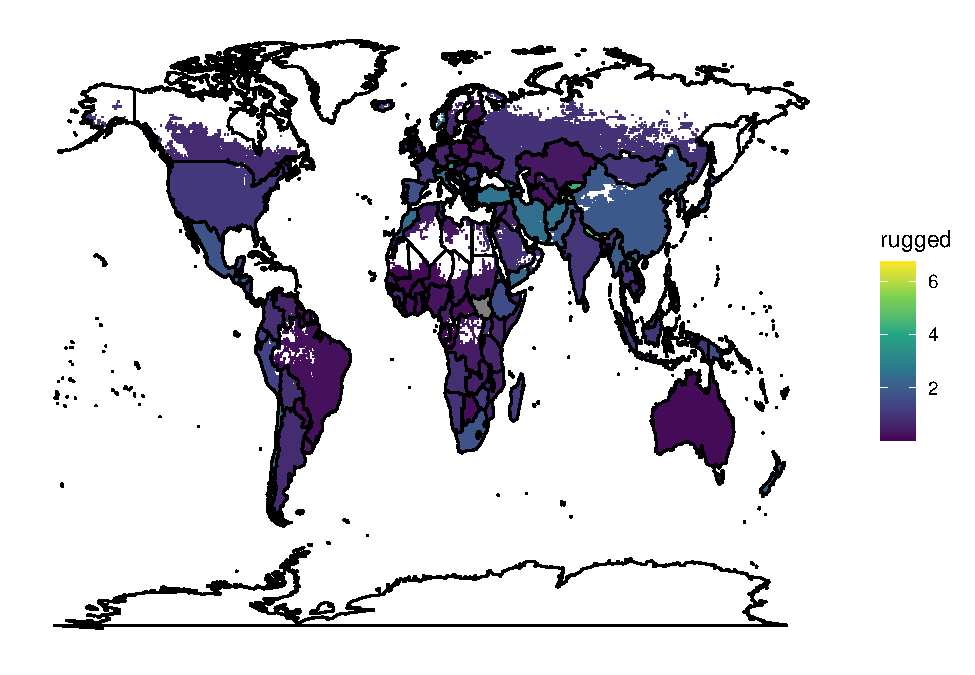
\includegraphics{thesis_files/figure-latex/TRI-1.pdf}
\caption{\label{fig:TRI}Terrain Ruggedness Index for the study area. TRI values}
\end{figure}
\hypertarget{dist}{%
\subsection{Compatibility: Distance to the Next Irrigated Cell}\label{dist}}

\hypertarget{distdata}{%
\subsubsection{LPJmL Derived Output}\label{distdata}}

\hypertarget{distdesc}{%
\subsubsection{Description}\label{distdesc}}

\hypertarget{popdens}{%
\subsection{Social Influences: Population Density}\label{popdens}}

\hypertarget{HYDE}{%
\subsection{History Database of the Global Environment}\label{HYDE}}

The History Database of the Global Environment (HYDE)

\hypertarget{popdensdesc}{%
\subsubsection{Description}\label{popdensdesc}}

\hypertarget{gdppc}{%
\subsection{Economics: Income}\label{gdppc}}

\hypertarget{maddison}{%
\subsubsection{Maddison Project Database}\label{maddison}}

\hypertarget{gdppcdesc}{%
\subsubsection{Description}\label{gdppcdesc}}

\hypertarget{democracy}{%
\subsection{External Influences: Democracy}\label{democracy}}

\hypertarget{BRdemo}{%
\subsubsection{Bjørnskov-Rode Regime Data}\label{BRdemo}}

\hypertarget{demodesc}{%
\subsubsection{Description}\label{demodesc}}

The base dataset used for this thesis was constructed as an input for LPJmL. A combination of global irrigation patterns from t(\protect\hyperlink{ref-schaphoffLPJmL4DynamicGlobal2018}{Schaphoff et al., 2018}). This dataset was then fed into LPJmL to and used to derive different variables including irrigation, cropland, and crop fraction on a per grid cell basis.

\hypertarget{hypothesis}{%
\section{Hypothesis}\label{hypothesis}}

Based on information discussed above several hypothesis can be formed to investigate the expected effects of different predictors. As discussed previously there are two outcome variables in this masters thesis: the presence/absence of irrigation and the amount of irrigation. Hypothesis are similar for both predictor variables.
\begin{center}\rule{0.5\linewidth}{0.5pt}\end{center}

For the amount of irrigation present in a cell the stated hypothesis for this thesis are:
\begin{enumerate}
\def\labelenumi{\arabic{enumi}.}
\tightlist
\item
  A \textbf{decrease in precipitation} will result in an \textbf{increase in irrigation}.
\item
  A \textbf{decrease in population density} will result in an \textbf{increase in irrigation}.
\item
  An \textbf{increase in income (GDP per capita)} will result in an \textbf{increase in irrigation.}
\item
\end{enumerate}
\hypertarget{studyreg}{%
\section{Study Region}\label{studyreg}}

To be able to investigate the patterns of global historical irrigation expansion, the initial proposed study area encompassed the entirely of the globe's terrestrial land mass with recorded observations detailing every year for the 45-year study period. This constituted a data set of roughly three million observations. In an effort to decrease computation time, a logical reduction of the study area (and therefore data) was necessary.

Figure \ref{fig:irrfrac-2005} illustrates the pattern of irrigation at the last time step (2005) of the study period. It is notable that irrigation does not exist at all in some places such as the higher latitudes and the Sahara. These areas also contain no cropland, no managed grasslands, and no pastureland. Upon the logic that irrigation cannot expand into areas that contain no agricultural land (whether it be cropland, grassland, or pasture land), all cells which contained no agricultural land over the the course of the study period were removed, giving rise to the study area you see in figure \ref{fig:study-region-nocrop}.
\begin{figure}
\centering
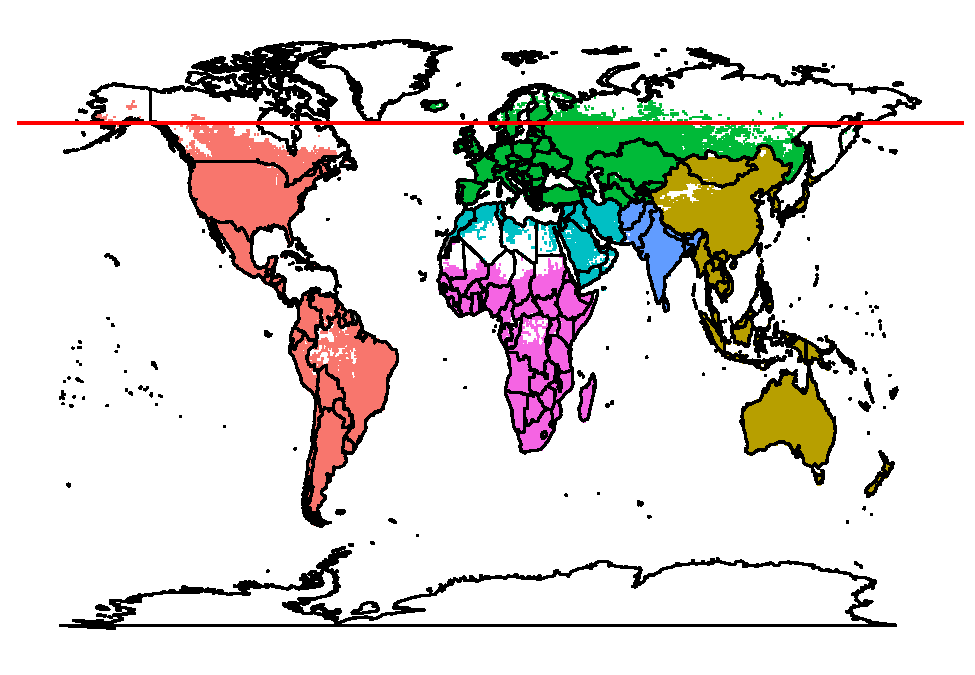
\includegraphics{thesis_files/figure-latex/study-region-nocrop-1.pdf}
\caption{\label{fig:study-region-nocrop}Final study area after the removal of cells with no agricultural land over the course of the 45 year study period. Colors represent regional groupings. Notice that excluded areas are located within the Amazon, the Sahara, Central Africa, the Middle East, Eastern China, and toward the Arctic Circle (represented at 60 degrees North with a red horozontal line).}
\end{figure}
\hypertarget{section-1}{%
\section{}\label{section-1}}

Building from the conceptual basis established in Section \ref{drivers} several hypothesis can be formed regarding the effects of various drivers on irrigation fraction.

\hypertarget{bayesintro}{%
\section{Modeling}\label{bayesintro}}

\hypertarget{thin}{%
\subsection{Thinning}\label{thin}}

\hypertarget{nocrop}{%
\subsubsection{Thinning for Conceptual Clarity}\label{nocrop}}

\hypertarget{autocorr}{%
\subsubsection{Thinning for Autocorrelated Structures}\label{autocorr}}

\emph{``The first law of geography: Everything is related to everything else, but near things are more related than distant things.'' - Walter Tobler (\protect\hyperlink{ref-toblerComputerMovieSimulating1970}{Tobler, 1970})}

Bayesian inference has some unique features in comparison to other forms of statistical influence. For the context of this thesis the two main advantages or Bayesian Inference are an improved propagation of uncertainty throughout the modeling process and an ability to include prior information into models, allowing the inclusion prior knowledge (\protect\hyperlink{ref-gelmanRegressionOtherStories2020}{Gelman, Hill, \& Vehtari, 2020}).

\hypertarget{bayesthe}{%
\subsection{Bayes Theorem}\label{bayesthe}}

Bayes' theorem is the basis for Bayesian inference. Although Bayes' theorem can be manipulated in to many forms, the most basic representation is Equation \eqref{eq:bayesmath}.
\begin{equation}
p(\theta|y) = \frac{ p(y|\theta) * p(\theta)}{p(y)}
\label{eq:bayesmath}
\end{equation}
Where \(\theta\) is an unknown parameter to be estimated and \(y\) is the observed data. To understand the what is happening here, it is necessary to define some terms using accessible language from \protect\hyperlink{ref-mcelreathStatisticalRethinkingBayesian2020}{McElreath} (\protect\hyperlink{ref-mcelreathStatisticalRethinkingBayesian2020}{2020, p. 37}).
\begin{itemize}
\item
  The symbol \textbar{} can be read as ``given'' or ``conditional on,'' meaning that the probability of one event is dependent on the occurrence of another. This is also known ask ``Conditional Probability.''
\item
  The outcome \(p(\theta|y)\), is also known as the ``posterior'' and can be read as ``the probability of a the unobserved parameter given the observed data.''
\item
  \(p(y|\theta)\) is the probability of the data, or the likelihood.
\item
  \(p(\theta)\), represents previous knowledge about the unobserved parameter \(\theta\), and is called the ``prior.''
\item
  \(p(y)\) is the ``average probability of the data,'' which is ``the probability of the data, that has been averaged over \(p(\theta)\),'' as \protect\hyperlink{ref-mcelreathStatisticalRethinkingBayesian2020}{McElreath} (\protect\hyperlink{ref-mcelreathStatisticalRethinkingBayesian2020}{2020, p. 37}) mentions. The main function of \(p(y)\) is to normalize the posterior (remember, \(p(\theta|y)\)).
\end{itemize}
All together Bayes' theorem looks like this (\protect\hyperlink{ref-mcelreathStatisticalRethinkingBayesian2020}{McElreath, 2020}):
\begin{equation}
\text{Posterior} = \frac{\text{Probability of the Data} * \text{Prior}}{\text{Average Probability of the Data}}
\label{eq:bayesword}
\end{equation}
It is important to remember that although Bayes' theorem can be used with point estimates\footnote{A point estimate is a single value, generally the average, given as the estimate value for a parameter.}, the advantage of Bayesian inference is that all terms in Equation \eqref{eq:bayesmath} can be represented as probability distributions, communicating much more uncertainty about a parameter than point estimate statistics. From this point forward, assume that terms such as posterior, prior, and likelihood imply distributions not point estimates. For fun, a relevant example of a point estimate use of Bayes Theorem is listed in Section \ref{covidex}.

Even more so when using probability distributions, often times it is difficult to deal with the normalizing term, \(p(y)\). However, as \(p(y)\) does not depend on the unobserved parameter \(\theta\), it can be considered a constant and factored out giving rise to the more common used and less computationally difficult \emph{unnormalized posterior density} (\protect\hyperlink{ref-gelmanBayesianDataAnalysis2013}{Gelman et al., 2013}; \protect\hyperlink{ref-mcelreathStatisticalRethinkingBayesian2020}{McElreath, 2020})\emph{.}
\begin{equation}
p(\theta|y) \propto p(y|\theta) * p(\theta)
\label{eq:proppost}
\end{equation}
Effectively, Equation \eqref{eq:proppost} means that the posterior is proportional to the likelihood, \(p(y|\theta)\), multiplied by the prior, \(p(\theta)\). Its not necessary in most contexts to normalize using \(p(y)\), proportionality works just fine.

\hypertarget{the-prior}{%
\subsubsection{The Prior}\label{the-prior}}

Specification of the prior distribution is not a trivial task, as the prior attempts to encapsulate the previous knowledge of a specific parameter and has impacts on the posterior distribution. The determination of the prior should be done before seeing the data and serves two main functions, communicating previous scientific or common knowledge about a parameters distribution and/or helping the the model learn more efficiently (\protect\hyperlink{ref-mcelreathStatisticalRethinkingBayesian2020}{McElreath, 2020}). Often times flat priors are used initially and improved upon iteratively. Effects of the prior on the posterior can be seen in Figure \ref{fig:prioreffects} which is adapted from \protect\hyperlink{ref-mcelreathStatisticalRethinkingBayesian2020}{McElreath} (\protect\hyperlink{ref-mcelreathStatisticalRethinkingBayesian2020}{2020, p. 38}) and \protect\hyperlink{ref-kurzStatisticalRethinkingBrms2019}{Kurz} (\protect\hyperlink{ref-kurzStatisticalRethinkingBrms2019}{2019, sec. 2.4}).
\begin{figure}
\centering
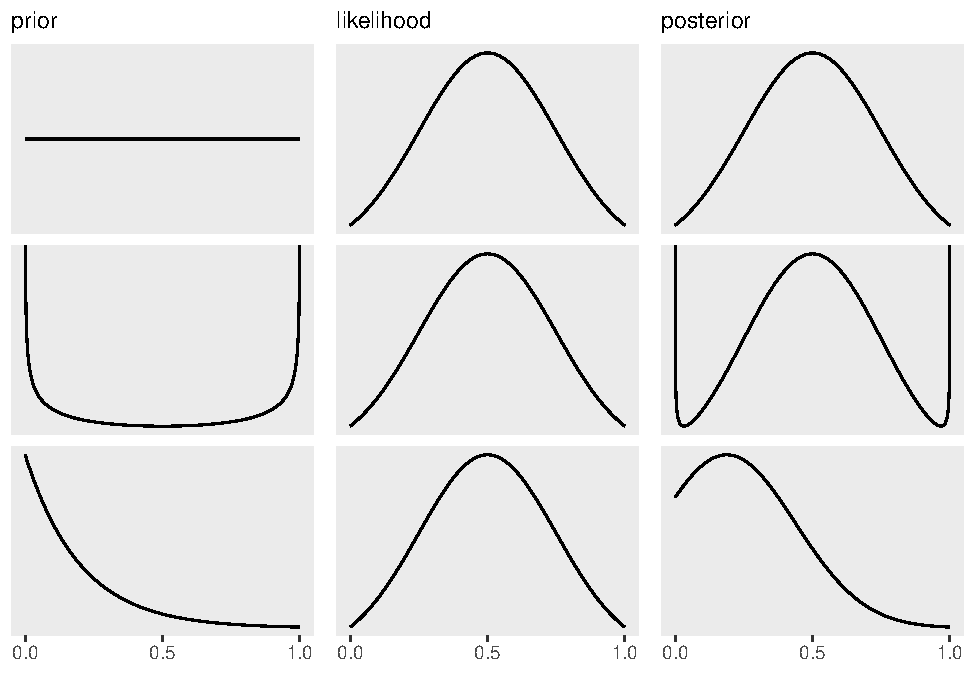
\includegraphics{thesis_files/figure-latex/prioreffects-1.pdf}
\caption{\label{fig:prioreffects}Effects of the prior distrubution on the unnormalized posterior with a Normal(0.5, 0.25) likelihood. First row: Uniform prior, Second row: Beta(a = 0.75, b = 0.75) prior, Third Row: Exponential prior. Prior and likelihood are multiplied together to create the unnormalized posterior seen in the third column.}
\end{figure}
There are several different types of priors used when discussing Bayesian inference. Some of the most common types of priors discussed are (\protect\hyperlink{ref-gelmanBayesianDataAnalysis2013}{Gelman et al., 2013}):
\begin{itemize}
\item
  \textbf{Proper priors,} which integrate to 1 and \textbf{improper priors,} that don't. The fact that a prior (or any probability distribution for that matter) integrates to 1 is important not only computationally, as it makes it easier to manipulate and solve analytically, but an improper prior violates the assumption that probability distributions integrate to 1.
\item
  \textbf{Informative priors} communicate information about a given parameter's distribution, \textbf{non-informative priors} do not. A classic example of a non informative prior is a flat or uniform prior (seen in the row 1 of Section \ref{fig:prioreffects}) as it assumes that all probability values are equally likely which is almost never the case.
\item
  To discuss the amount of information communicated via the prior distribution to the posterior, terms such as \textbf{Strongly Informative Priors} or \textbf{Weakly Informative Priors} can be used. Weakly informative priors are informative (i.e.~they do contain information about the distribution of a given parameter) but serve to regularize the posterior only by setting bounds within which the posterior can vary its shape, meaning that they are not aiming to completely describe the distribution of a parameter. In addition, these priors are easily overwhelmed if the amount of data is large. Strongly informative priors, conversely, heavily influence the posterior distribution and are more likely to overwhelm the data.
\end{itemize}
The goal when specifying the prior is to have at least a weakly informative prior for each given parameter. This ensures that general scientific knowledge about the distribution of a parameter is communicated but if large amounts of data exist, the prior gives way to the overwhelming evidence of the likelihood (\protect\hyperlink{ref-gelmanPriorChoiceRecommendations2020}{Gelman, 2020}). Manipulation of the prior can be useful from can be used to solve or diagnose issues, given certain contexts and questions. However, it is important to note that ``bad'' (less suitable) priors can come with some unintended consequences such as allowing for more unstable predictions due sampling difficulties from bad geometry of the posterior (when using tools such as STAN (\protect\hyperlink{ref-standevelopmentteamRStanInterfaceStan2020}{Stan Development Team, 2020})) or entertaining predictions that are not possible given the problem (ex. predicting negative values when logically only positive ones exist) (\protect\hyperlink{ref-mcelreathStatisticalRethinkingBayesian2020}{McElreath, 2020, sec. 5.1}). Priors that are skeptical of extreme values are often times called \emph{regularizing} priors (\protect\hyperlink{ref-mcelreathStatisticalRethinkingBayesian2020}{McElreath, 2020, sec. 7.5})

\protect\hyperlink{ref-gelmanPriorCanOften2017}{Gelman, Simpson, \& Betancourt} (\protect\hyperlink{ref-gelmanPriorCanOften2017}{2017}) and \protect\hyperlink{ref-gelmanPriorChoiceRecommendations2020}{Gelman} (\protect\hyperlink{ref-gelmanPriorChoiceRecommendations2020}{2020}) discuss appropriate prior choice and emphasize that the identification of weak or strong priors is not possible without knowledge of the likelihood, which violates the idea that a prior should be constructed \emph{a priori,} or before having any notion of the data or even the data generating process. As mentioned in \protect\hyperlink{ref-gelmanPriorCanOften2017}{Gelman, Simpson, \& Betancourt} (\protect\hyperlink{ref-gelmanPriorCanOften2017}{2017, sec. 1.2}), this may be the most ideal way to construct a prior but in reality practical concerns such as model convergence, unknown parameters, knowledge of the modeler, etc. make this task impossible or very difficult. Hence, a division is created that separates Bayesian issues into two camps, those can/are willing to build a prior in a \emph{subjective} way by incorporating expert/scientific knowledge into the prior \emph{before} seeing the data or setting up the model, and those that ``break'' this rule by using some knowledge about the likelihood and data to construct their prior.

Ultimately, prior specification for Bayesian inference is necessary but is often times more of an art than a science. Iterative processes help with choosing the prior and seeing its effect on the posterior for a given question, dataset, and model. The overall aim is to balance practical and theoretical concerns when choosing most the suitable prior. Currently, a large area of research focuses solely on prior specification and usage within a Bayesian context aimed at demystifying prior specification and increasing standardization of prior specification processes and documentation.

\hypertarget{model-comparison}{%
\subsection{Model Comparison}\label{model-comparison}}

Multiple ways to compare models exist, some rely more heavily on a conceptual and causal understanding of the problem, others rely on predictive accuracy. Model comparison can occur \emph{within-sample} or \emph{out-of-sample,} meaning that comparisons calculated using data used to train the model (\emph{within-sample}) or using data that has been left our when fitting the model (\emph{out-of-sample}).

More informal methods of model comparison exist such as prior and posterior predictive checks, comparison of bayes' factor or bayesian \(R^2\) among others. (\protect\hyperlink{ref-gelmanUnderstandingPredictiveInformation2014}{Gelman, Hwang, \& Vehtari, 2014}). However, as these checks are done using within-sample data, and some can be prone to overfitting under certain circumstances (\protect\hyperlink{ref-mcelreathStatisticalRethinkingBayesian2020}{McElreath, 2020, Chapter 7})

\hypertarget{hierarchical-modeling}{%
\subsection{Hierarchical Modeling}\label{hierarchical-modeling}}

\hypertarget{dags}{%
\subsubsection{DAGs}\label{dags}}

A Directed Acyclic Graph (DAG)
\begin{figure}
\centering
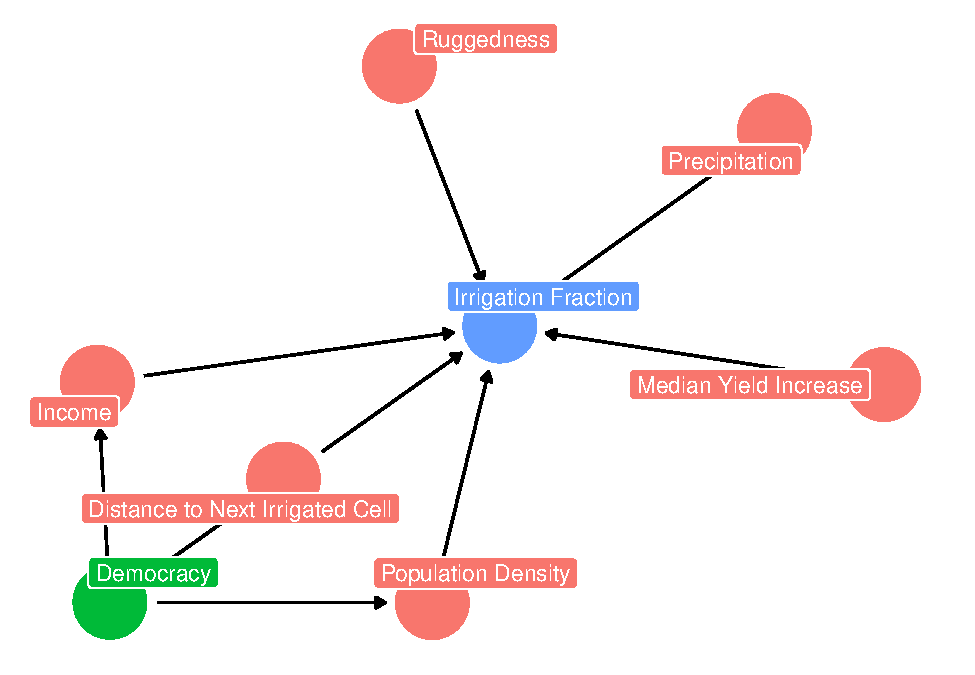
\includegraphics{thesis_files/figure-latex/mudag-1.pdf}
\caption{\label{fig:mudag}Directed Acyclic Graph for Beta}
\end{figure}
\begin{figure}
\centering
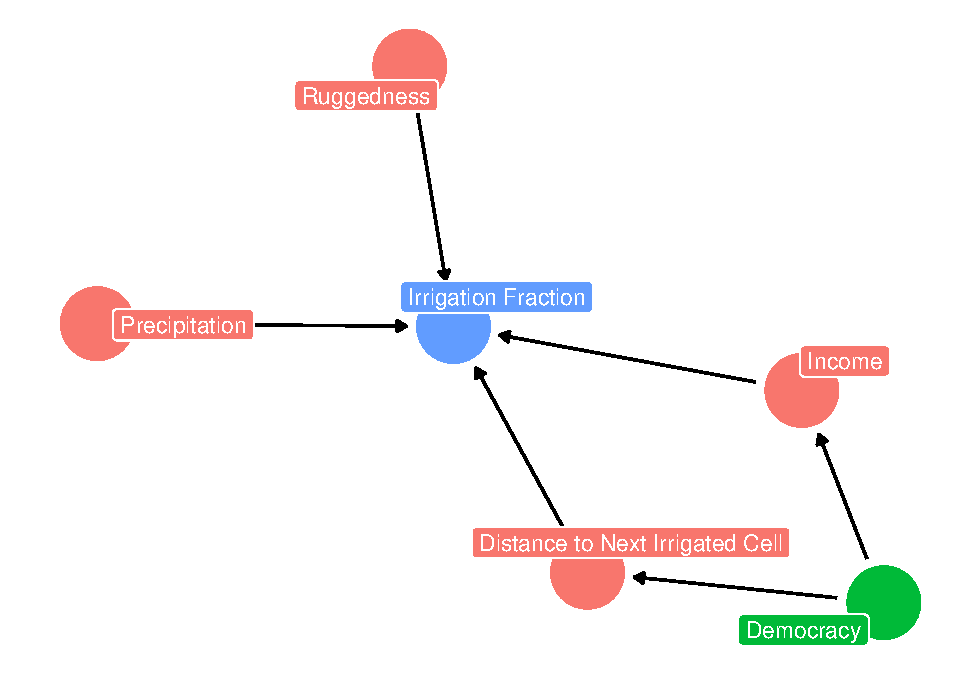
\includegraphics{thesis_files/figure-latex/zidag-1.pdf}
\caption{\label{fig:zidag}Directed Acyclic Graph for zero inflated paramater zi}
\end{figure}
To test these hypothesis, a quick view of correlations was carried out.

\texttt{fr\ if(knitr:::is\_latex\_output())\ \textquotesingle{}\textbackslash{}\textbackslash{}appendix\textquotesingle{}}

\hypertarget{appendix}{%
\chapter{Appendix}\label{appendix}}

\hypertarget{bayesproof}{%
\section{\texorpdfstring{Proof of Bayes' Theorem for Two Hypothesis from \protect\hyperlink{ref-hackingIntroductionProbabilityInductive2001}{Hacking} (\protect\hyperlink{ref-hackingIntroductionProbabilityInductive2001}{2001})}{Proof of Bayes' Theorem for Two Hypothesis from Hacking (2001)}}\label{bayesproof}}

Definition of \textbf{Conditional Probability} taken from \protect\hyperlink{ref-hackingIntroductionProbabilityInductive2001}{Hacking} (\protect\hyperlink{ref-hackingIntroductionProbabilityInductive2001}{2001}) beginning on p.49:
\begin{equation}
\text{Pr(A|B)}= \frac{\text{Pr(A,B)}}{\text{Pr(B)}} 
\label{eq:conditionalprob}
\end{equation}
Implying that for \(\text{Pr(B) > 0}\),
\begin{equation}
\text{Pr(A|B)} * \text{Pr(B)} = \text{Pr(A,B)}  
\label{eq:conditionalprobproof1}
\end{equation}
Knowing that,
\begin{equation}
\text{Pr(B,A)} = \text{Pr(A,B)} 
\label{eq:conditionalprobproof2}
\end{equation}
Therefore,
\begin{equation}
\text{Pr(B|A)} * \text{Pr(A)} = \text{Pr(A|B)} * \text{Pr(B)} 
\label{eq:conditionalprobproof3}
\end{equation}
Dividing by \(\text{P(A)}\), gives Bayes' Theorem (equivalent to Equation \eqref{eq:bayesmath})
\begin{equation}
\text{Pr(B|A)}= \frac{\text{Pr(A|B) * Pr(B)}}{\text{Pr(A)}} 
\label{eq:bayes}
\end{equation}
Assuming that \(0 < \text{Pr(B)} < 1\), the equation for \textbf{Total Probability} taken from \protect\hyperlink{ref-hackingIntroductionProbabilityInductive2001}{Hacking} (\protect\hyperlink{ref-hackingIntroductionProbabilityInductive2001}{2001, p. 59}) can be written:
\begin{equation}
\text{Pr(A)} = \text{Pr(A|B)} * \text{Pr(B)} + \text{Pr(A|Not B)} * \text{Pr(Not B)}
\label{eq:totalprob}
\end{equation}
Substituting Equation \eqref{eq:totalprob} into Equation \eqref{eq:bayes}, giving rise to the Equation \eqref{eq:twohypothesis}, the base equation used for the basis of Equation \eqref{eq:bayesspecial},
\begin{equation}
\text{Pr(B|A)}= \frac{\text{Pr(A|B) * Pr(B)}}{\text{Pr(A|B)} * \text{Pr(B)} + \text{Pr(A|Not B)} * \text{Pr(Not B)}} 
\label{eq:twohypothesis}
\end{equation}
\hypertarget{covidex}{%
\section{Digression: Covid Rapid Antigen Tests}\label{covidex}}

Imagine (you don't have to) that SARS-CoV-2 is circulating in Berlin. An individual takes a rapid antigen test and receives a positive test result. However, the media recently has been discussing that rapid antigen tests are less accurate than other types of tests to detect SARS-CoV-2, like the PCR. The individual thinks that perhaps the test was wrong, meaning that this person received a ``false positive'' and doesn't actually have Covid even though the test came back positive. Data can be gathered, a positive test result (the \(y\)), and a hypothesis can be constructed, the individual doesn't have Covid (the \(\theta\)). Substituting this in to Bayes' theorem, the probability that this individual doesn't have Covid even though the test came back positive can be calculated (remember, \(p(\theta|y)\)) using Equation \eqref{eq:covidword}.
\begin{equation}
\text{p(No Covid|Pos)} = \frac{\text{p(Pos|No Covid)} * \text{p(No Covid)}}{\text{p(Pos)}}
\label{eq:covidword}
\end{equation}
Some extra information is necessary to fill in the missing pieces,
\begin{itemize}
\item
  According to \protect\hyperlink{ref-tagesspiegelCoronavirusKarteDeutschlandweiteFallzahlen2021}{Tagesspiegel} (\protect\hyperlink{ref-tagesspiegelCoronavirusKarteDeutschlandweiteFallzahlen2021}{2021}), 200 people are infected with SARS-CoV-2 for every 100,000 people in Berlin, also known as probability of having Covid (\(\text{P(Covid)} = 0.002\)). Since our hypothesis is that the individual \emph{doesn't} have Covid, we can calculate \(\text{P(No Covid)} = 0.998\). This represents our previous knowledge about how many people don't have Covid and is the prior (\(p(\theta)\)) in Bayes' theorem.
\item
  My local \href{https://schnell.coronatest.de/?lang=en}{Covid Test Center} claims that their rapid antigen tests have a sensitivity of 96\% and a specificity of 99\%. Sensitivity is the ability to correctly identify those who have the disease and specificity is the ability to correctly identify those that do not have the disease.
  \begin{itemize}
  \tightlist
  \item
    So sensitivity represents the probability of testing positive when (or \emph{given}) you have Covid, \(\text{P(Positive|Covid)} = 0.96\). Conversely, the \(\text{P(Negitive|Covid)} = 0.04\)
  \item
    Specificity represents the probability of testing negative given you don't have Covid \(\text{P(Negative|No Covid)} = 0.99\). Then, \(\text{P(Positive|No Covid)} = 0.01\). This is the probability of the data, or the likelihood \((p(y|\theta))\).
  \end{itemize}
\end{itemize}
From these statements, Table \ref{tab:makingcovid} can be created .
\begin{table}[H]

\caption{\label{tab:makingcovid}\label{tab:makingcovid}Probabilities for incidence of Covid and rapid antigen test sensitivity.}
\centering
\begin{tabular}[t]{lll}
\toprule
  & Covid (p = 0.002) & No Covid (p = 0.998)\\
\midrule
Positive & 0.96 & 0.01\\
Negative & 0.04 & 0.99\\
\bottomrule
\end{tabular}
\end{table}
Last thing that needs to be discussed is the denominator, \(\text{p(Positive)}\) or \(p(y)\). There is a manipulation of Bayes's rule using the law of Conditional Probability detailed in \protect\hyperlink{ref-hackingIntroductionProbabilityInductive2001}{Hacking} (\protect\hyperlink{ref-hackingIntroductionProbabilityInductive2001}{2001}) that can be used in cases where there are only two outcomes (two \(\theta\)s ). This can be applied here as is this the case, i.e.~the person either has or doesn't have Covid. Equation (\protect\hyperlink{ref-ref}{\textbf{ref?}})(eq:bayesspecial) details \protect\hyperlink{ref-hackingIntroductionProbabilityInductive2001}{Hacking} (\protect\hyperlink{ref-hackingIntroductionProbabilityInductive2001}{2001}) for this example. Proof for (\protect\hyperlink{ref-ref}{\textbf{ref?}})(eq:bayesspecial) can be seen in \ref{bayesproof}.
\begin{equation}
P(\text{No Covid|Pos}) = \frac{\text{P(Pos|No Covid)} * \text{P(No Covid)}}{\text{P(Pos|No Covid)} * \text{P(No Covid)} + \text{P(Pos|Covid)} * \text{P(Covid)}}
\label{eq:bayesspecial}
\end{equation}
From then using Table \ref{tab:makingcovid} and Equation \eqref{eq:bayesspecial}, the probability of not having Covid given a positive test result can be calculated.
\begin{align}
P(\text{No Covid|Pos}) &= \frac{0.01 * 0.998}{0.01 * 0.998 + 0.96 * 0.002} \\
P(\text{No Covid|Pos}) &= 0.84
\label{eq:bayesmath2}
\end{align}
So, what does this mean? This \(\text{P(No Covid|Pos)} = 0.84\) is the probability of not having Covid given a positive test result. This is quite high, so chances are even though the test came back positive, this individual does not have Covid. Perhaps we should take another rapid test or a PCR.

\hypertarget{predselect}{%
\section{Predictor Selection}\label{predselect}}

\backmatter

\hypertarget{references}{%
\chapter*{References}\label{references}}
\addcontentsline{toc}{chapter}{References}

\markboth{References}{References}

\noindent

\setlength{\parindent}{-0.20in}
\setlength{\leftskip}{0.20in}
\setlength{\parskip}{8pt}

\hypertarget{refs}{}
\begin{CSLReferences}{1}{0}
\leavevmode\hypertarget{ref-adachiAgriculturalTechnologiesTerraced2007}{}%
Adachi, S. (2007). Agricultural {Technologies} of {Terraced Rice Cultivation} in the {Ailao Mountains}, {Yunnan}, {China}, \emph{6}(2), 173--196. http://doi.org/\href{https://doi.org/10.14956/asafas.6.173}{10.14956/asafas.6.173}

\leavevmode\hypertarget{ref-angelakisIrrigationWorldAgricultural2020}{}%
Angelakis, A. N., Zaccaria, D., Krasilnikoff, J., Salgot, M., Bazza, M., Roccaro, P., \ldots{} Fereres, E. (2020). Irrigation of {World Agricultural Lands}: Evolution through the {Millennia}. \emph{Water}, \emph{12}(5), 1285. http://doi.org/\href{https://doi.org/10.3390/w12051285}{10.3390/w12051285}

\leavevmode\hypertarget{ref-bjornebergIRRIGATIONMethods2013}{}%
Bjorneberg, D. L. (2013). {IRRIGATION} \textbar{} {Methods}. In \emph{Reference {Module} in {Earth Systems} and {Environmental Sciences}}. {Elsevier}. http://doi.org/\href{https://doi.org/10.1016/B978-0-12-409548-9.05195-2}{10.1016/B978-0-12-409548-9.05195-2}

\leavevmode\hypertarget{ref-europeancomissionEurostatDatabase2021}{}%
Comission, E. (2021). Eurostat {Database}. https://ec.europa.eu/eurostat/data/database.

\leavevmode\hypertarget{ref-faoStateWorldLand2011}{}%
FAO. (2011). \emph{The state of the world's land and water resources for food and agriculture ({SOLAW}) {} {Managing} systems at risk}. {Rome and London}: {FAO and Earthscan}.

\leavevmode\hypertarget{ref-faoAQUASTAT2021}{}%
FAO. (2021a). {AQUASTAT}. http://www.fao.org/aquastat/en/databases/.

\leavevmode\hypertarget{ref-faoFAOSTAT2021}{}%
FAO. (2021b). {FAOSTAT}. http://www.fao.org/faostat/en/\#data.

\leavevmode\hypertarget{ref-faoIrrigationWaterManagement1985}{}%
FAO, Brouwer, C., Goffeau, A., \& Heibloem, M. (1985). \emph{Irrigation {Water Management}: Introduction to {Irrigation}}. {Rome}.

\leavevmode\hypertarget{ref-faoIrrigationWaterManagement1986a}{}%
FAO, Brouwer, C., \& Heibloem, M. (1986). \emph{Irrigation {Water Management}: Irrigation {Water Needs}}. {Rome}.

\leavevmode\hypertarget{ref-faoIrrigationWaterManagement1986}{}%
FAO, Brouwer, C., Prins, K., Kay, M., \& Heibloem, M. (1986). \emph{Irrigation {Water Management}: Irrigation {Methods}} (No. Training Manual no. 5). {Rome}.

\leavevmode\hypertarget{ref-faoIrrigationManualPlanning2001}{}%
FAO, \& SAFR. (2001). \emph{Irrigation manual: Planning, development, monitoring and evaluation of irrigated agriculture with farmer participation}. {Harare}: {Food and Agriculture Organization of the United Naitons (FAO), Sub-Regional Office for East and Southern Africa (SAFR)}.

\leavevmode\hypertarget{ref-faoGuidelinesDesigningEvaluating1989}{}%
FAO, \& Walker, W. R. (1989). \emph{Guidelines for designing and evaluating surface irrigation systems}. {Rome}.

\leavevmode\hypertarget{ref-forsethTerrestrialBiomes2010}{}%
Forseth, I. (2010). Terrestrial {Biomes}. \emph{Nature Education Knowledge}. https://www.nature.com/scitable/knowledge/library/terrestrial-biomes-13236757/.

\leavevmode\hypertarget{ref-gelmanPriorChoiceRecommendations2020}{}%
Gelman, A. (2020, April). Prior {Choice Recommendations}. \emph{Stan Dev GitHub}. https://github.com/stan-dev/stan/wiki/Prior-Choice-Recommendations.

\leavevmode\hypertarget{ref-gelmanBayesianDataAnalysis2013}{}%
Gelman, A., Carlin, J. B., Stern, H. S., Dunson, D. B., Vehtari, A., \& Rubin, D. B. (2013). \emph{Bayesian {Data Analysis}}. {Chapman and Hall/CRC}. http://doi.org/\href{https://doi.org/10.1201/b16018}{10.1201/b16018}

\leavevmode\hypertarget{ref-gelmanRegressionOtherStories2020}{}%
Gelman, A., Hill, J., \& Vehtari, A. (2020). \emph{Regression and {Other Stories}}. {Cambridge University Press}.

\leavevmode\hypertarget{ref-gelmanUnderstandingPredictiveInformation2014}{}%
Gelman, A., Hwang, J., \& Vehtari, A. (2014). Understanding predictive information criteria for {Bayesian} models. \emph{Statistics and Computing}, \emph{24}(6), 997--1016. http://doi.org/\href{https://doi.org/10.1007/s11222-013-9416-2}{10.1007/s11222-013-9416-2}

\leavevmode\hypertarget{ref-gelmanPriorCanOften2017}{}%
Gelman, A., Simpson, D., \& Betancourt, M. (2017). The {Prior Can Often Only Be Understood} in the {Context} of the {Likelihood}. \emph{Entropy}, \emph{19}(10), 555. http://doi.org/\href{https://doi.org/10.3390/e19100555}{10.3390/e19100555}

\leavevmode\hypertarget{ref-hackingIntroductionProbabilityInductive2001}{}%
Hacking, I. (2001). \emph{An {Introduction} to {Probability} and {Inductive Logic}}. http://doi.org/\href{https://doi.org/10.1017/CBO9780511801297}{10.1017/CBO9780511801297}

\leavevmode\hypertarget{ref-holzapfelIrrigationAgriculture2008}{}%
Holzapfel, E. A., \& Mariño, M. A. (2008). Irrigation in {Agriculture}. In S. E. Jørgensen \& B. D. Fath (Eds.), \emph{Encyclopedia of {Ecology}} (pp. 2033--2039). {Oxford}: {Academic Press}. http://doi.org/\href{https://doi.org/10.1016/B978-008045405-4.00628-5}{10.1016/B978-008045405-4.00628-5}

\leavevmode\hypertarget{ref-kleingoldewijkHundredYear18901997}{}%
Klein Goldewijk, C., \& Battjes, J. (1997). A {Hundred Year} (1890 - 1990) {Database} for {Integrated Environmental Assessments} ({HYDE}, version 1.1). \emph{PBL Netherlands Environmental Assessment Agency}.

\leavevmode\hypertarget{ref-kurzStatisticalRethinkingBrms2019}{}%
Kurz, A. S. (2019). \emph{Statistical {Rethinking} with brms, Ggplot2, and the tidyverse}.

\leavevmode\hypertarget{ref-mcelreathStatisticalRethinkingBayesian2020}{}%
McElreath, R. (2020). \emph{Statistical {Rethinking}: A {Bayesian Course} with {Examples} in {R} and {STAN}} (Second). {Chapman and Hall/CRC}.

\leavevmode\hypertarget{ref-neumannExploringGlobalIrrigation2011}{}%
Neumann, K., Stehfest, E., Verburg, P. H., Siebert, S., Müller, C., \& Veldkamp, T. (2011). Exploring global irrigation patterns: A multilevel modelling approach. \emph{Agricultural Systems}, \emph{104}(9), 703--713.

\leavevmode\hypertarget{ref-pikLPJmLLundPotsdamJenaManaged}{}%
PIK. (n.d.). {LPJmL} - {Lund}-{Potsdam}-{Jena} managed {Land} {} {Potsdam Institute} for {Climate Impact Research}. https://www.pik-potsdam.de/en/institute/departments/activities/biosphere-water-modelling/lpjml.

\leavevmode\hypertarget{ref-portmannMIRCA2000GlobalMonthly2010a}{}%
Portmann, F. T., Siebert, S., \& Döll, P. (2010). {MIRCA2000}{{Global}} monthly irrigated and rainfed crop areas around the year 2000: A new high-resolution data set for agricultural and hydrological modeling. \emph{Global Biogeochemical Cycles}, \emph{24}(1). http://doi.org/\href{https://doi.org/10.1029/2008GB003435}{10.1029/2008GB003435}

\leavevmode\hypertarget{ref-worldwaterassesnentprogramUnitedNationsWorld2009}{}%
Program, W. W. A., \& UNESCO. (2009). \emph{The {United Nations World Water Development Report} 3: Water in a {Changing World}}. {Paris}.

\leavevmode\hypertarget{ref-puyCurrentModelsUnderestimate2020}{}%
Puy, A., Lo Piano, S., \& Saltelli, A. (2020). Current {Models Underestimate Future Irrigated Areas}. \emph{Geophysical Research Letters}, \emph{47}(8), e2020GL087360. http://doi.org/\href{https://doi.org/10.1029/2020GL087360}{10.1029/2020GL087360}

\leavevmode\hypertarget{ref-rileyTerrainRuggednessIndex1999}{}%
Riley, S., Degloria, S., \& Elliot, S. D. (1999). A {Terrain Ruggedness Index} that {Quantifies Topographic Heterogeneity}. \emph{Internation Journal of Science}, \emph{5}, 23--27.

\leavevmode\hypertarget{ref-rockstromManagingWaterRainfed2010}{}%
Rockström, J., Karlberg, L., Wani, S. P., Barron, J., Hatibu, N., Oweis, T., \ldots{} Qiang, Z. (2010). Managing water in rainfed agriculture{{The}} need for a paradigm shift. \emph{Agricultural Water Management}, \emph{97}(4), 543--550. http://doi.org/\href{https://doi.org/10.1016/j.agwat.2009.09.009}{10.1016/j.agwat.2009.09.009}

\leavevmode\hypertarget{ref-schaphoffLPJmL4DynamicGlobal2018}{}%
Schaphoff, S., Von Bloh, W., Rammig, A., Thonicke, K., Biemans, H., Forkel, M., \ldots{} Waha, K. (2018). {LPJmL4} - {A} dynamic global vegetation model with managed land - {Part} 1: Model description. \emph{Geoscientific Model Development}, \emph{11}(4), 1343--1375. http://doi.org/\href{https://doi.org/10.5194/gmd-11-1343-2018}{10.5194/gmd-11-1343-2018}

\leavevmode\hypertarget{ref-siebertGroundwaterUseIrrigation2010}{}%
Siebert, S., Burke, J., Faures, J. M., Frenken, K., Hoogeveen, J., Döll, P., \& Portmann, F. T. (2010). Groundwater use for irrigation {} a global inventory. \emph{Hydrology and Earth System Sciences}, \emph{14}(10), 1863--1880. http://doi.org/\href{https://doi.org/10.5194/hess-14-1863-2010}{10.5194/hess-14-1863-2010}

\leavevmode\hypertarget{ref-siebertGlobalDataSet2015}{}%
Siebert, Stefan, Kummu, M., Porkka, M., Döll, P., Ramankutty, N., \& Scanlon, B. (2015). A global data set of the extent of irrigated land from 1900 to 2005. \emph{Hydrology and Earth System Sciences}, \emph{19}, 1521--1545. http://doi.org/\href{https://doi.org/10.5194/hess-19-1521-2015}{10.5194/hess-19-1521-2015}

\leavevmode\hypertarget{ref-standevelopmentteamRStanInterfaceStan2020}{}%
Stan Development Team. (2020). {RStan}: The {R} interface to {Stan}.

\leavevmode\hypertarget{ref-tagesspiegelCoronavirusKarteDeutschlandweiteFallzahlen2021}{}%
Tagesspiegel. (2021, May). Coronavirus-{Karte}: Deutschlandweite {Fallzahlen} in {Echtzeit}. \emph{Tagesspiegel}. https://interaktiv.tagesspiegel.de/lab/karte-sars-cov-2-in-deutschland-landkreise/.

\leavevmode\hypertarget{ref-thenkabailGlobalIrrigatedArea2009}{}%
Thenkabail, P. S., Biradar, C. M., Noojipady, P., Dheeravath, V., Li, Y., Velpuri, M., \ldots{} Dutta, R. (2009). Global irrigated area map ({GIAM}), derived from remote sensing, for the end of the last millennium. \emph{International Journal of Remote Sensing}, \emph{30}(14), 3679--3733. http://doi.org/\href{https://doi.org/10.1080/01431160802698919}{10.1080/01431160802698919}

\leavevmode\hypertarget{ref-toblerComputerMovieSimulating1970}{}%
Tobler, W. R. (1970). A {Computer Movie Simulating Urban Growth} in the {Detroit Region}. \emph{Economic Geography}, \emph{46}, 234. http://doi.org/\href{https://doi.org/10.2307/143141}{10.2307/143141}

\leavevmode\hypertarget{ref-universityofeastangliaclimaticresearchunitVersionCRUTS2021}{}%
University of East Anglia Climatic Research Unit, Harris, I., Osborn, T. J., \& Jones, P. (2021). Version 4 of the {CRU TS} monthly high-resolution gridded multivariate climate dataset. \emph{Scientific Data}, \emph{7}(1), 109. http://doi.org/\href{https://doi.org/10.1038/s41597-020-0453-3}{10.1038/s41597-020-0453-3}

\end{CSLReferences}

% Index?

\end{document}
